\documentclass{article}
\usepackage[utf8]{inputenc}
\usepackage{geometry}
\usepackage{pdfpages}
\usepackage{filecontents}
\graphicspath{{images/}}
\geometry{
	a4paper,
	total={170mm,257mm},
	left=20mm,
	top=20mm,
}
\usepackage{graphicx}
\usepackage{titling}
\usepackage[american,RPvoltages]{circuiTikz}
\usepackage{tikz, tikz-cd}
\usepackage{pgfplots}
\usepackage{siunitx}
\usepackage{float}
\usepackage{enumitem}
\usepackage{amsmath,amsfonts,stmaryrd,amssymb} % Math packages
\usepackage{schemabloc}
\usepackage{tcolorbox}
\usepackage{xcolor}

\title{Circuito con diodo con carga $\mathrm{R}$-$\mathrm{L}$}
\author{Rodrigo}
\date{Agosto 2024}

\usepackage{fancyhdr}
\fancypagestyle{plain}{%  the preset of fancyhdr 
	\fancyhf{} % clear all header and footer fields
	\fancyfoot[L]{\thedate}
	\fancyhead[L]{Diodo con carga RL}
	\fancyhead[R]{\theauthor}
}
\makeatletter
\def\@maketitle{%
	\newpage
	\null
	\vskip 1em%
	\begin{center}%
		\let \footnote \thanks
		{\LARGE \@title \par}%
		\vskip 1em%
		%{\large \@date}%
	\end{center}%
	\par
	\vskip 1em}
\makeatother

\usepackage{lipsum}  
\usepackage{cmbright}
\renewcommand{\figurename}{Figura}
%---------------------------------------------------
\tikzset{flipflop myRS/.style={flipflop,
		flipflop def={t1=R, t3=S, t6=Q, t4={\ctikztextnot{Q}}, tu={\ctikztextnot{RST}}, nu=1, n4=1 }}
}

\tikzset{flipflop myFFRS/.style={flipflop,
		flipflop def={t1=R, t3=S, t6=Q, t4={\ctikztextnot{Q}}, n4=1 }}
}
%---------------------------------------------------

\makeatletter
\newcommand*{\underarrow}{\def\@underarrow{\relax}\@ifstar{\@@underarrow}{\def\@underarrow{\hidewidth}\@@underarrow}}
\newcommand*{\@@underarrow}[2][]{\underset{\@underarrow\substack{\uparrow\if\relax\detokenize{#1}\relax\else\\#1\fi}\@underarrow}{#2}}

\newcommand*{\overarrow}{\def\@overarrow{\relax}\@ifstar{\@@overarrow}{\def\@overarrow{\hidewidth}\@@overarrow}}
\newcommand*{\@@overarrow}[2][]{\overset{\@overarrow\substack{\if\relax\detokenize{#1}\relax\else#1\\\fi\downarrow}\@overarrow}{#2}}
\makeatother

\begin{document}
	
	\maketitle
	
	\noindent\begin{tabular}{@{}ll}
		Author & \theauthor\\
		Chapter &  2 - Power diodes and Switched RLC Circuits \\
		Book & Power Electronics, devices, circuits and applications \\
		Page & pp. 80
	\end{tabular}
	
	\section*{Circuito con carga RL}
	En la siguiente figura se muestra un circuito con diodo en el cual se conecta una carga $RL$. Asuma que $v_s = V_m \sin (\omega t) \, \mathrm{V}$. Cuando el interruptor $S_1$ se cierra en el tiempo $t=0$ la corriente a través del inductor puede ser expresada como 
	
	\begin{figure}[H]
		\centering	
		\begin{tikzpicture}[scale=0.8]
			\def\x{2.1*pi}% scalebar-x at golden ratio of x=1728px
			\def\y{320}% scalebar-y at 90% of height of y=356px
			\ctikzset{bipoles/thickness=3}
			\ctikzset{monopoles/vcc/arrow={Stealth[width=6pt,length=9pt]}}
			\ctikzset{monopoles/vee/arrow={Stealth[width=6pt,length=9pt]}}
			\draw (0,0) to[sV, l=$v_s$] ++(0,6)
			to[ccgsw, l=$S_1$, a=${t=0}$] ++(3,0)
			to[D, i_=$i_L$, l=$D_1$] ++(3,0) coordinate (p1)
			to[R, l_=$R$, v^=$v_R$] ++(0,-3)
			to[L,l_=$L$, v^=$v_L$] ++(0,-3)
			to[short] (0,0);
			%\draw (p1)++(2,0) to[open, v_=$v_O$] ++(0,-6);
		\end{tikzpicture}
		\caption{}	
		\label{fig:figura1}
	\end{figure}
	
\begin{align}
	v_s - v_R - v_L = 0
\end{align}

\noindent La relación $v$-$i$ de un inductor está dada por
\begin{align}
	v_L = L \frac{di_L}{dt}
\end{align}

\noindent Y la relación $v$-$i$ de un resistor es:
\begin{align}
	v_R = Ri_L
\end{align}

\noindent La sustitución de (2) y (3) en (1) produce

\begin{align}
	L \frac{di_L}{dt} + Ri_L = V_m \sin (\omega t)
\end{align}

\section*{Introducción a las ecuaciones lineales}
Un tipo de ecuación diferencial de primer orden que ocurre frecuentemente en diversas aplicaciones es la ecuación lineal, una \textbf{ecuación lineal de primer orden} puede ser expresada en la forma

\begin{align}
	a_1(x) \frac{dy}{dx} + a_0(x)y = b(x)
\end{align}

\noindent Donde $a_1(x)$, $a_0(x)$ y $b(x)$ dependen sólo de la variable independiente $x$, no de $y$

\noindent La forma más fácil de ordenar una ecuación diferencial de primer orden es colocarla en su \textbf{forma estándar}, esto se logra dividiendo la ecuación original (5) entre $a_1(x)$

\begin{tcolorbox}[colback=red!5!white,colframe=red!75!black,arc=0mm,boxrule=0mm,width=(\linewidth+0.5cm)]
	\begin{equation}
		\frac{dy}{dx} + P(x)y = Q(x)
	\end{equation}
\end{tcolorbox}

\noindent Donde $P(x) = a_0(x)/a_1(x)$ y $Q(x) = b(x)/a_1(x)$ \\

\noindent El siguiente paso es determinar $\mu (x)$ de tal manera que el lado izquiero de la ecuación (6) sea la derivada del producto $\mu(x)y$:

\begin{align}
	\mu(x)\frac{dy}{dx} + \color{cyan} \mu(x)P(x) \color{black} y = \frac{d}{dx} \left[ \mu(x)y \right] = \mu(x) \frac{dy}{dx} + \color{cyan} \mu'(x) \color{black} y
\end{align}

\noindent Claramente, esto requiere que $\mu$ satisfaga

\begin{align}
	\mu' = \mu P
\end{align}

\noindent Para encontrar dicha función, reconocemos que (8) es una ecuación diferencial separable  la cual puede escribirse como

\begin{align}
	\frac{d\mu}{dx} = \mu P(x) \nonumber \\
	\frac{d\mu}{\mu} = P(x)dx \noindent
\end{align}

\noindent Al integrar ambos lados obtenemos

\begin{tcolorbox}[colback=red!5!white,colframe=red!75!black,arc=0mm,boxrule=0mm,width=(\linewidth+0.5cm)]
	\begin{equation}
		\mu (x) = e^{\int{P(x)dx}}
	\end{equation}
\end{tcolorbox}

\noindent Con esta elección para $\mu (x)$, la ecuación (7) se vuelve

\begin{align}
	\frac{d}{dx}[\mu (x)y] = \mu (x)Q(x) \nonumber
\end{align}

\noindent La cual tiene la siguiente solución

\begin{align}
	y(x) = \frac{1}{\mu (x)} = \left[ \int \mu (x)Q(x) dx + C \right]
\end{align}

\begin{tcolorbox}[colback=red!5!white,colframe=red!75!black,arc=0mm,boxrule=0mm,width=(\linewidth+0.5cm),title=Método para resolver ecuaciones lineales,colbacktitle=red!60!white,coltitle=white]
	\begin{enumerate}[] 
		\item Escriba la ecuación en su forma estándar
		\begin{equation}
			\frac{dy}{dx} + P(x)y = Q(x) \nonumber
		\end{equation}
		\item Calcule el factor de integración $\mu(x)$ mediante la fórmula
		\begin{equation}
			\mu(x) = e^{\int P(x) dx} \nonumber
		\end{equation}
		\item Multiplique la ecuación en su forma estándar por $\mu(x)$, y recuerde que el lado izquierdo es sólo $\frac{d}{dx}[\mu(x)y]$ para obtener
		\begin{align}
			\underbrace{\mu(x)\frac{dy}{dx} + P(x)\mu(x)y } &= \mu(x)Q(x) \nonumber \\
			\frac{d}{dx}[\mu(x)y]  \qquad &= \mu(x)Q(x) \nonumber
		\end{align}
		\item Integre la última ecuación y resuelva para $y$ dividiendo por $\mu(x)$ para obtener (11)
	\end{enumerate}
\end{tcolorbox}

\section*{Encontrando la solución general}
Una vez sentadas las bases para resolver una ecuación diferencial de primer orden, el primer paso es colcoar (4) en su forma estándar, esto es

\begin{align}
	\frac{di_L}{dt} + \frac{R}{L}i_L = \frac{V_m}{L}\sin(\omega t)
\end{align}

\noindent 
\begin{align}
	P(x) = \frac{R}{L} \nonumber
\end{align}

\noindent Así, el factor de integración es

\begin{align}
	\mu(t) = e^{\int \frac{R}{L} dt} = e^{\frac{R}{L}t}
\end{align}

\noindent Multiplicamos (13) en ambos lados de la ecuación en (12)

\begin{align}
	\underbrace{e^{\frac{R}{L}t} \frac{di_L}{dt} + \frac{R}{L}e^{\frac{R}{L}t}i_L} &= \frac{V_m}{L}e^{\frac{R}{L}t}\sin(\omega t) \nonumber \\
	\frac{d}{dt}(e^{\frac{R}{L}t} i_L) \quad &= \frac{V_m}{L}e^{\frac{R}{L}t}\sin(\omega t) \nonumber
\end{align}

\noindent Ahora integramos ambos lados y resolvemos para $i_L$

\begin{align}
	\int d(e^{\frac{R}{L}t} i_L) = \frac{V_m}{L} \int e^{\frac{R}{L}t}\sin(\omega t) \, dt  \nonumber \\
	e^{\frac{R}{L}t} i_L = \frac{V_m}{L} \int e^{\frac{R}{L}t}\sin(\omega t) \, dt
\end{align}

\noindent Para resolver la integral en (14), la cual es conocida como integral por partes podemos usar el siguiente método de integración

\subsection*{Integración tabular}
Es bien sabido que las integrales de la forma $\int f(x)g(x) \, dx$, en las que $f$ se deriva de forma repetida hasta volverse cero y $g$ se integra varias veces sin dificultad, son candidatas naturales para integración por partes. Sin embargo, si se requieren muchas repeticiones, los cálculos puedes volverse pesados. En situaciones como ésta, existe una manera de organizar los cálculos que evita estas fallas y hace el trabajo mucho más sencillo, el cual se denomina \textbf{integración tabular}. La integración tabular también se aplica a integrales de la forma  $\int f(x)g(x) \, dx$ cuando ninguna de las dos funciones puede derivarse de manera repetida hasta convertirse cero. \\

\noindent Para resolver estos tipos de integración por partes, construimos una tabla que lista las derivadas sucesivas de $f(x)$ y las integrales de $g(x)$ como se muestra a continuación:

\begin{figure}[H]
	\centering	
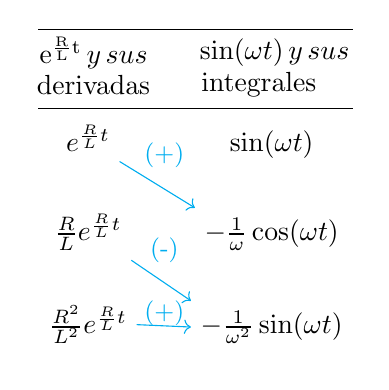
\begin{tikzpicture}
	\matrix (m) [matrix of math nodes, nodes in empty cells]
	{
		e^{\frac{R}{L}t} &  &  &  & \sin(\omega t) \\
		 				 &  &  &  &                \\
		 				 &  &  &  & 			   \\
		\frac{R}{L} e^{\frac{R}{L}t} &  &  &  & - \frac{1}{\omega} \cos (\omega t) \\
		 				 &  &  &  & 			   \\
						 &  &  &  & 			   \\
		\frac{R^2}{L^2} e^{\frac{R}{L}t} &  &  &  & - \frac{1}{\omega^2} \sin (\omega t) \\		
	};
	\draw[->, cyan] (m-1-1.south east) -- (m-4-5.north west);
	\draw[->, cyan] (m-4-1.south east) -- (m-7-5.north west);
	\draw[->, cyan] (m-7-1.east) -- (m-7-5.west);
	\node[cyan] at (-0.4,1){\small(+)};
	\node[cyan] at (-0.4,-0.2){\small(-)};
	\node[cyan] at (-0.4,-1){\small(+)};
	\node[] at(-1.3,2.3){$\mathrm{e^{\frac{R}{L}t}} \, y \, sus$};
	\node[] at(-1.3,1.9){$\mathrm{derivadas}$};
	\node[] at(1,2.3){$\sin (\omega t) \, y \, sus$};
	\node[] at(0.8,1.9){$\mathrm{integrales}$};
	\draw (-2,1.6) -- (2,1.6);
	\draw (-2,2.6) -- (2,2.6);
\end{tikzpicture}
	\caption{}	
	\label{fig:figura2}
\end{figure}

\noindent De la tabla de la figura anterior, nos detenemos hasta que el $n$-ésimo renglón sea el mismo que el primero (salvo por las constantes multiplicativas). Interpretamos la tabla diciendo que:

\begin{align}
	\int e^{\frac{R}{L}t}\sin(\omega t) \, dt = -\frac{1}{\omega} e^{\frac{R}{L}t} \cos (\omega t) + \frac{R}{\omega^2 L} e^{\frac{R}{L}t} \sin (\omega t) - \frac{R^2}{\omega^2 L^2} \int e^{\frac{R}{L}t} \sin (\omega t) \, dt \nonumber \\
	\left( 1 + \frac{R^2}{\omega^2 L^2} \right) \int e^{\frac{R}{L}t}\sin(\omega t) \, dt = -\frac{1}{\omega} e^{\frac{R}{L}t} \cos (\omega t) + \frac{R}{\omega^2 L} e^{\frac{R}{L}t} \sin (\omega t) \nonumber \\
	\left( \frac{\omega^2 L^2 + R^2}{\omega^2 L^2} \right) 	\int e^{\frac{R}{L}t}\sin(\omega t) \, dt =-\frac{1}{\omega} e^{\frac{R}{L}t} \cos (\omega t) + \frac{R}{\omega^2 L} e^{\frac{R}{L}t} \sin (\omega t) \nonumber \\
	\int e^{\frac{R}{L}t}\sin(\omega t) \, dt = -\left( \frac{1}{\omega} \right) \left( \frac{\omega^2 L^2}{\omega^2 L^2 + R^2} \right)e^{\frac{R}{L}t} \cos (\omega t) + \left( \frac{R}{\omega^2 L} \right) \left( \frac{\omega^2 L^2}{\omega^2 L^2 + R^2} \right) e^{\frac{R}{L}t} \sin (\omega t) \nonumber
\end{align}

\noindent Al simplificar un poco obtemos

\begin{align}
	\int e^{\frac{R}{L}t}\sin(\omega t) \, dt = - \left( \frac{\omega L^2}{\omega^2 L^2 + R^2} \right) e^{\frac{R}{L}t} \cos (\omega t) +  \left(\frac{RL}{\omega^2 L^2 + R^2} \right) e^{\frac{R}{L}t} \sin (\omega t) \nonumber
\end{align}

\noindent Al traer de vuelta la constante multiplicativa $\frac{V_m}{L}$ a la integral, obtenemos:

\begin{align}
	\frac{V_m}{L} \int e^{\frac{R}{L}t}\sin(\omega t) \, dt = V_m e^{\frac{R}{L}t} \left[ - \left( \frac{\omega L}{\omega^2 L^2 + R^2} \right) \cos (\omega t) + \left(\frac{R}{\omega^2 L^2 + R^2} \right) \sin (\omega t) \right] + C
\end{align}

\noindent Podemos simplificar aún más la ecuación en (15) expresando el término $\alpha \sin(x) - \beta \cos(x)$ como $R \sin (x - \theta)$ utilizando la siguiente identidad trigonométrica:

\noindent Sea 

\begin{align}
	\sin (x - \theta) &= \sin x \cos \theta - \cos x \sin \theta \nonumber \\
	R \left[ \sin (x - \theta) \right] &= R[\sin x \cos \theta - \cos x \sin \theta] \nonumber \\
	&= R\sin x \cos \theta - R \cos x \sin \theta \nonumber \\
	&= (R \cos \theta)\sin x - (R \sin \theta) \cos x \nonumber
\end{align}

\noindent Donde

\begin{align}
	a = R \cos \theta \nonumber \\
	b = R \sin \theta \nonumber
\end{align}

\noindent Si elevamos ambos términos al cuadrado obtenemos

\begin{align}
	a^2 + b^2 &= R^2 \cos^2 \theta + R^2 \sin^2 \theta \nonumber \\
	&= R^2 \left[  \sin^2 \theta + \cos^2 \theta \right] \nonumber \\
	a^2 + b^2 &= R^2 \nonumber
\end{align}

\noindent Al despejar para $R$ obtenemos

\begin{align}
	R = \sqrt{a^2 + b^2} \nonumber
\end{align}

\noindent De la ecuación en (15), sea:

\begin{align}
	a = \frac{R}{\omega^2 L^2 + R^2} \nonumber \\
	b = \frac{\omega L}{\omega^2 L^2 + R^2} \nonumber
\end{align}

\noindent Así, el valor de $R$ está dado por

\begin{align}
	R &= \sqrt{\frac{R^2}{ \left[ \omega^2 L^2 + R^2 \right]^2} +  \frac{\omega^2 L^2}{ \left[ \omega^2 L^2 + R^2 \right]^2} } \nonumber \\
	&= \sqrt{ \frac{R^2 + \omega^2 L^2}{ \left[ \omega^2 L^2 + R^2 \right]^2} } \nonumber \\
	&= \frac{1}{\omega^2 L^2 + R^2} \nonumber
\end{align}

\noindent Por último, la ecuación en (15) se puede escribir como

\begin{align}
		\frac{V_m}{L} \int e^{\frac{R}{L}t}\sin(\omega t) \, dt = \frac{V_m}{\sqrt{  \omega^2 L^2 + R^2 }} e^{\frac{R}{L}t} \sin (\omega t - \theta) + C
\end{align}

\noindent Donde

\begin{align}
	\theta = \arctan{\frac{\omega L}{R}}
\end{align}

\noindent Una vez encontrada la integral, retornamos a la ecuación (14), al sustituir (16) en (14) y despejamos para $i_L$ obtenemos

\begin{align}
	i_L  = \frac{V_m}{\sqrt{  \omega^2 L^2 + R^2 }} \sin (\omega t - \theta) + Ce^{-\frac{R}{L}t}, \quad i_L(0) = I_0
\end{align}

\noindent Para encontrar el valor de la constante de integración, hacemos uso de la condición inicial con lo cual obtenemos
\begin{align}
	i_L(0) = \frac{V_m}{\sqrt{  \omega^2 L^2 + R^2 }} \sin ( - \theta) + Ce^{0} = I_0 \nonumber \\
	C = I_0 -  \frac{V_m}{\sqrt{  \omega^2 L^2 + R^2 }} \sin ( - \theta) \nonumber \\
	C = I_0 +  \frac{V_m}{\sqrt{  \omega^2 L^2 + R^2 }} \sin (\theta)
\end{align}

\noindent La sustitución de (19) en (18) da como resultado

\begin{tcolorbox}[colback=red!5!white,colframe=red!75!black,arc=0mm,boxrule=0mm,width=(\linewidth+0.5cm)]
	\begin{equation}
			i_L(t)  = \frac{V_m}{\sqrt{  \omega^2 L^2 + R^2 }} \sin (\omega t - \theta) + \left( I_0 +  \frac{V_m}{\sqrt{  \omega^2 L^2 + R^2 }} \sin \theta \right) e^{-\frac{R}{L}t}
	\end{equation}
\end{tcolorbox}


\end{document}